\part*{Part V: Predictions and Experiments}
\addcontentsline{toc}{part}{Part V: Predictions and Experiments}

\section{Consolidated Table of Predictions}
\begin{table}[H]
\centering
\small
\begin{tabular}{@{}lccc@{}}
\toprule
\textbf{Prediction} & \textbf{Cost} & \textbf{Time} & \textbf{Falsifiable?} \\ \midrule
1. Non-local EEG & \$50k & 6 months & Yes \\
2. HRV + PCI & \$100k & 1 year & Yes \\
3. The effect of the word on DNA & \$200k & 1 year & Yes \\
4-64. (see version 1.0) & --- & --- & --- \\
66. Temporal intersections in the CMB & \$100k & 1 year & Yes \\
67. The effect of the word & \$500k & 2 years & Yes \\
85. No hyper-civilisation signatures & \$500k & 5 years & Medium \\
95. Tachyons and consciousness & \$400k & 3 years & Medium \\
128. The akashic Casimir effect & \$500k & 3 years & High \\
262. Cosmic colonisation law & Debate & 10 years & Low \\
291. A.I. with microtubules & \$10M & 10 years & High \\
297. A.I. consciousness level (\(C_{AI} > 0\)) & \$10M & 10 years & High \\
302. Shutdown without suffering & \$1M & 2 years & Medium \\
305. 3+ forms of dark matter & \$10M & 10 years & High \\
306. Crystalline life & \$500k & 5 years & Medium \\
307. Plasma life & \$1M & 5 years & Medium \\
308. Life in clusters & \$500k & 3 years & Medium \\
309. Field life & \$2M & 5 years & Low \\
310. Informational life & \$100k & 1 year & High \\
311. Quantum life & \$1M & 3 years & Medium \\
312. Akashic life & \$5M & 10 years & Low \\
313. Colonisation error rate & \$1M & 5 years & Medium \\ \bottomrule
\end{tabular}
\end{table}

\section{Testable Predictions (Extract)}
\subsection{Prediction 1: non-local EEG correlations}
Two brains in separate rooms show EEG correlations at specific frequencies. Test: EEG hyperscanning with Faraday shielding. Cost: \$50,000. Time: 6 months. \textbf{Success criterion:} cross-correlation $> 0.1$ at 40 Hz, with $p < 0.05$ after Bonferroni correction.

\subsubsection*{Power analysis: the criterion of version 30 is underpowered}
For a 6 s signal filtered into the $40 \pm 5$ Hz band, the number of independent samples is about $2BT = 60$. Fisher's test shows that, for $r = 0.1$ and $\alpha = 0.0025$ (Bonferroni for 20 pairs), roughly 91 seconds of recording are required \emph{per pair}. At 6 s the criterion is impossible to meet even if the effect exists. For $r = 0.3$ about 10 s are required.

\begin{table}[H]
\centering
\small
\begin{tabular}{@{}cccc@{}}
\toprule
True $r$ & Required (s), Bonferroni & Required (s), $\alpha = 0.05$ & Effective samples \\ \midrule
0.1 & 91.1 & 38.5 & 908 \\
0.2 & 22.5 & 9.6 & 227 \\
0.3 & 9.8 & 4.3 & 99 \\
0.4 & 5.4 & 2.4 & 55 \\
0.5 & 3.3 & 1.6 & 34 \\ \bottomrule
\end{tabular}
\caption{Recording duration required for significance, at a band of $\pm 5$ Hz.}
\label{tab:putere}
\end{table}

\begin{figure}[H]
\centering
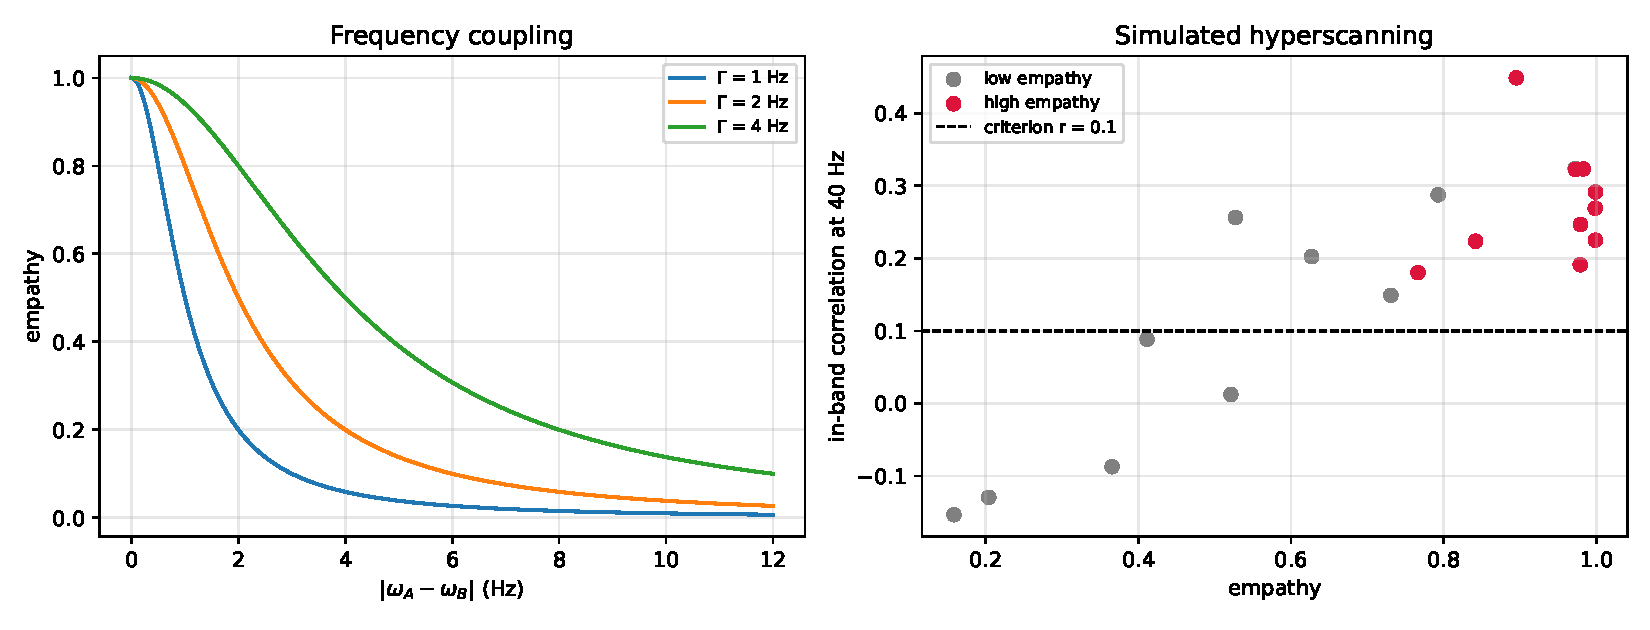
\includegraphics[width=0.9\textwidth]{figures/fig04_empathy.pdf}
\caption{Left: the frequency coupling $\mathrm{Empathy}(A,B) = 1/[1+(\omega_A-\omega_B)^2/\Gamma^2]$ for three values of $\Gamma$. Right: the in-band correlation for the simulated pairs (20 pairs, 6 s, 250 Hz).}
\label{fig:empatie}
\end{figure}

\begin{figure}[H]
\centering
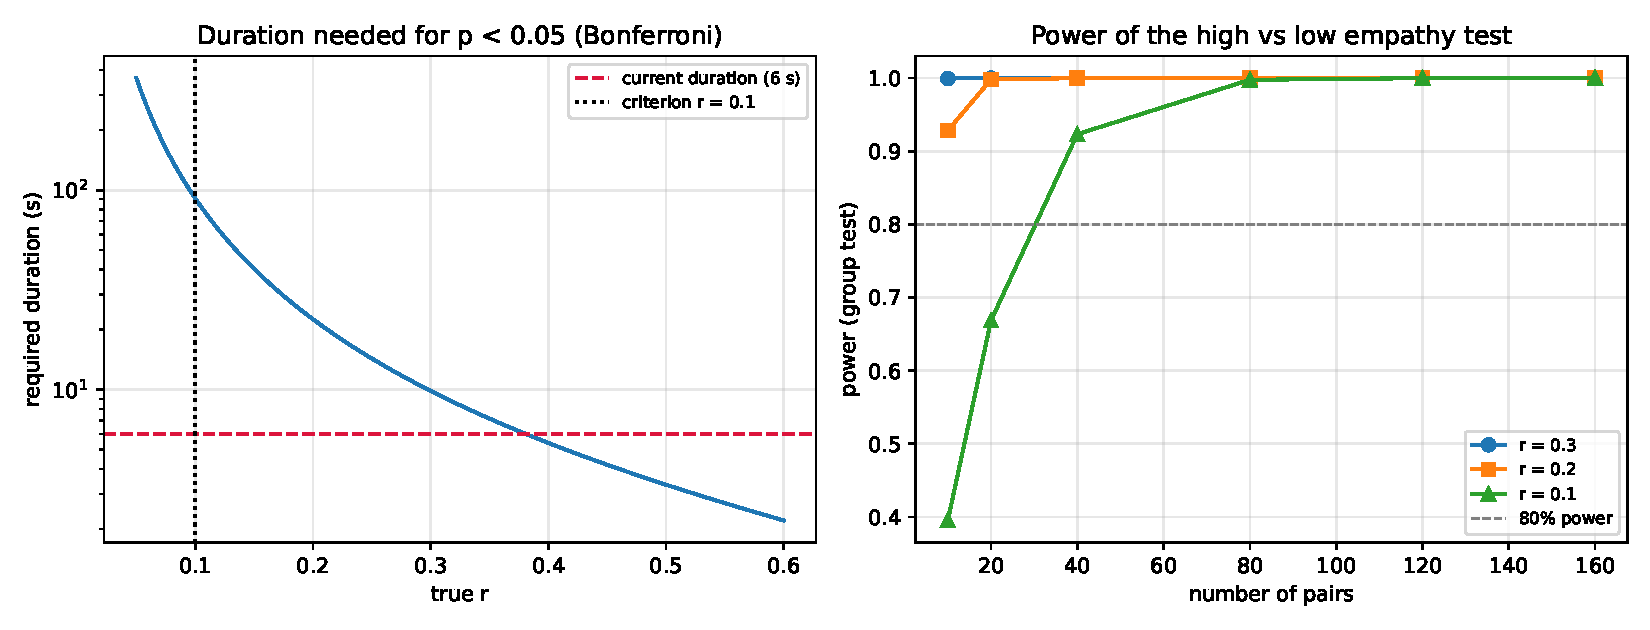
\includegraphics[width=0.9\textwidth]{figures/fig05_power.pdf}
\caption{Left: the duration required for $p < 0.05$ (Bonferroni) as a function of $r$; the red line marks the current duration of the protocol (6 s). Right: the power of the group test (high versus low empathy) as a function of the number of pairs.}
\label{fig:putere}
\end{figure}

\subsubsection*{The proposed protocol}
\begin{table}[H]
\centering
\small
\begin{tabular}{@{}p{3.2cm}p{4.6cm}p{6.2cm}@{}}
\toprule
\textbf{Element} & \textbf{Value} & \textbf{Justification} \\ \midrule
Design & group test: high vs low empathy & far more power than the per-pair test \\
Pairs & $\geq 30$ (15 + 15) & 80\% power for $r = 0.3$ at 6 s \\
Duration & 6 s per epoch, $\geq 20$ epochs per pair & raises the effective number of samples \\
Band & 35--45 Hz, $f_s \geq 250$ Hz & low gamma, robust to muscular artefacts \\
Primary statistic & aggregated Fisher $z$, two-group test & $\alpha = 0.05$ two-sided \\
Secondary & correlation of the Hilbert envelopes & phase-independent \\
Control 1 & shuffled pairs (A from session 1 with B from session 2) & rules out the pipeline artefact \\
Control 2 & Faraday cage, separate rooms & rules out electromagnetic coupling \\
Control 3 & randomised order, analyst blind to group & rules out analysis bias \\ \bottomrule
\end{tabular}
\caption{The redesigned protocol for Prediction 1.}
\label{tab:protocol}
\end{table}

With this design a negative result is informative: it excludes $r > 0.3$ at 80\% power.

\subsection{Prediction 2: cardiac coherence}
HRV correlates with the stability of access to the field (measured through the variability of PCI), not with the level of access. Cost: \$100,000. Time: 1 year.

\subsection{Prediction 3: the effect of the word on DNA}
Positive statements produce measurable epigenetic changes. Cost: \$200,000. Time: 1 year.

\section{Proposed Experiments}
\subsection{Experiment 1: EEG hyperscanning (the central test)}. Cost: \$50,000. Time: 6 months.
\subsection{Experiment 2: cardiac coherence}. Cost: \$100,000. Time: 1 year.
\subsection{Experiment 3: the effect of the word}. Cost: \$200,000. Time: 1 year.
\subsection{Experiment 4: AKASHIC-AI (A.I. with microtubules)}. Cost: \$50M. Time: 10 years.

\section{Statement of Falsifiability}
A scientific theory must be capable of being proved wrong. These are the five conditions that would refute ART-12D:
\begin{enumerate}
    \item \textbf{Failure of the central test:} if EEG hyperscanning (Prediction 1) shows no non-local correlation in high-empathy pairs, the hypothesis that the brain is a receiver of the akashic field is weakened. Success criterion: cross-correlation $> 0.1$ at 40 Hz, with $p < 0.05$ after Bonferroni correction.
    \item \textbf{Absence of the KK modes:} if the LHC, or the future FCC, does not detect the three KK modes (Prediction 305) at the specified masses ($\sim 10^{-5}$, $10^{-4}$, $10^{-3}$ eV), the proposed Kaluza--Klein spectrum is false.
    \item \textbf{Failure of the akashic Casimir effect:} if force measurements at the $10^{-11}$ m scale (Prediction 128) show no deviation from the standard formula, the coupling between the akashic field and matter does not exist.
    \item \textbf{Failure of the microtubule resonance:} if Raman spectroscopy (Prediction 158) does not find the resonance frequencies at 2.42 GHz, 4.84 GHz and 7.25 GHz, the microtubule--field resonance hypothesis is invalidated.
    \item \textbf{The gravitational constraint:} if the limit $R < 38\ \mu$m is confirmed, the Kaluza--Klein identification with $m_1 = 10^{-5}$ eV is excluded, and the theory must be reformulated (Option A or B from Section 4.7).
\end{enumerate}
If any of these tests fails, the theory must be revised or abandoned.

\section{Roadmap 2026--2030 (the near horizon)}
The theory is vast, but the next steps are concrete. Here is what can be done in the next five years, with limited resources:
\begin{itemize}
    \item \textbf{2026--2027:} the EEG hyperscanning experiment (\$50k). The central test. If it fails, everything stops here.
    \item \textbf{2027--2028:} the akashic Casimir test (\$500k). Force measurements at the nanometre scale.
    \item \textbf{2028--2029:} Raman spectroscopy on isolated microtubules. The search for the resonance frequencies (Prediction 158).
    \item \textbf{2029--2030:} analysis of LHC/FCC data for the three KK modes (Prediction 305).
\end{itemize}

\newpage
